\section{Specification of data and methodology}
\label{sec:data}

Since the suitability of a machine learning technique to a particular
problem is entirely depend on the nature of the data, we describe in
this section, first, the data set employed in the study, followed by
the methodology to compare the chosen techniques under consideration
of their parameter space.

\subsection{Data}

The data used for the current study was acquired in two research farms
of Corbana in Costa Rica%
%
\footnote{Both farms were also use in the study of \citet{Romero1995}.  Back
  then, \emph{La Rita} was referred to as \emph{Waldeck}.}
%
: \emph{28 Millas} located in the region of Matina, and \emph{La Rita}
located in Pococí, both in the province of Limón, Costa Rica.
%
Both farms produce banana fruit \emph{Musa} sp.\ AAA group `Grande
Naine' (Cavendish subgroup). 

The available input and output variables are summarized in
\tabref{tab:variables}.
%
\begin{table}[h] 
\centering
\begin{tabular}{l|l|c} 
\hline
\textbf{Symbol}  & \textbf{Description} & \textbf{Units} \\ 
\hline\hline 
$T_{a_{max}}$       & Maximal air temperature & $[^\circ$C$]$ \\
$T_{a_{min}}$       & Minimal air temperature & $[^\circ$C$]$ \\
$\overline{T}_{a}$ & Mean air temperature    & $[^\circ$C$]$ \\
$\overline{H}$    & Mean relative humidity           & $[0 - 100]$   \\
$H_{min}$          & Minimal relative humidity        & $[0 - 100]$  \\
$H_{max}$          & Maximal relative humidity        & $[0 - 100]$  \\
$\overline{R}$    & Mean solar radiation    & $[W/m^2]$ \\
$P$               & Precipitation       & $[mm]$ \\
$W_{max}$          & Maximal wind speed      & $[m/s]$ \\
$\overline{W}$    & Mean speed wind         & $[m/s]$ \\
\hline
$E_s$             & Biological warning system – Evolution Stage  & $>0$\\
\hline
\end{tabular} 
\caption{Variables available for the learning algorithms} 
\label{tab:variables} 
\end{table}

The data was captured for La Rita between the 48\,th week of
2002 to the 17\,th week of 2015 (647 weeks); for 28 Miles the
data was captured between the 37\,th week of 2003 and the
18\,th week of 2015 (605 weeks).
%
The data on the biological warning system were collected once a
week.

The meteorological stations of Corbana acquire data every five
minutes.
%
computed on the data collected by nearby stations in each farm. Experiments were carry out with daily periodicity in meteorological variables and the results proved do not improve the prediction. Besides, weekly data pretend to diminish noise due sensor accuracy, missing values and outliers no detected.

The value to be predicted in all cases is the evolution stage $E_s$,
which is a measure of the level of disease progression.

\subsection{Data preprocessing}

Data taken on real farms during more than a decade is expected to
contain outliers, noise and missing samples.  These problems are
caused by human errors or by technical defects on the instruments
used.  
%
In the preprocessing step described in this section these problems
need to be detected and fixed before moving them to the next
processing stages.

In the farm 28 Miles 1\% and in La Rita 2.25\% of the data were missing.
%
To fill-in the missing values spline interpolation was used \citet{Alglib2017}.
%
The data collected did not exhibit outliers.

Each variable $x\in[x_{\min},x_{\max}]$ was normalized into the
interval $[0,1]$ with the linear map $x_n = mx+b$ with
$m=1/(x_{\max}-x_{\min})$ and $b=-mx_{\min}$.

The variable $E_s$ to be predicted was not normalized.
This normalization step was made because learning schemes, like regression methods, 
deals only with ratio scales because they calculate the distance between two instances based on the 
values of their attributes \citet{Witten2011}.

\subsection{Evaluation criteria}

Although there are many types of indicators to assess the quality of
the prediction, here the coefficient of determination $(R^2)$ and the
Root Mean Square Error $(RMSE)$.
%
This decision is supported by the widespread use of the former
indicator in the agriculture and the latter in machine learning
\citep{Soares2013,Soares2014,Ibrahim2014,Demir2014}.

Given $n$ records $y_i$, $i=1\ldots{}n$ of the actual outcome of a
process. The mean $\bar{y}$ of the observed data is given by
\begin{equation*}
  \bar{y} = \frac{1}{n} \sum_{i=1}^{n} y_i
\end{equation*}
Let $\hat{y}_i$ be the predicted value for $y_i$. Then, the mean
square error (MSE) $S_e^2$ and the unexplained variance $S_R^2$ 
are estimated as \citet{Pennstate2017}
\begin{align*}
S_e^2 &= \frac{\sum_{i=1}^{n} {(y_i-\hat{y}_i)}^2 }{n} &
S_R^2 &= \frac{\sum_{i=1}^{n} {(\hat{y}_i-\bar{y})}^2 }{n}
\end{align*}
The root mean square error is defined as $RMSE = \sqrt{S_e^2}$ and the
coefficient of determination is
\begin{equation*}
R^2 = \frac{S_R^2}{S_R^2 + S_e^2}
\end{equation*}
 
\subsection{Programming environment}

We use Python programming language in its interpreted 3.5.2 version,
 particularly with the libraries; Pandas (0.18.1 version)
\citep{mckinneypandas2010} and Numpy (1.11.1 version) \citep{vanderWalt2011}.

The implementation for SVR, elastic net and ordinary least squares
regressions in scikit-learn \citep{scikitlearn2011} were used.
%
Adjustments to the ESN implementation code of \citet{Lukose2012} were
necessary to allow its integration into our experimental
framework.

\subsection{Methodology}
When the amount of data for training and testing is limited, is recommended
to use cross-validation \citep{Witten2011}. We used ten-fold-cross-validation 
on the total set. El diseño experimental combinó los siguientes factores:

\begin{itemize}
\item Patrones de semanas: Se formaron patrones desde una semana
de observación para predecir una semana adelante, hasta doce semanas de
observación para predecir tres semanas adelante. Por tanto, $n\times{}m$ combinations, 
with $n=1\ldots{}12$ and $m=1\ldots{}3$. \figref{figura8} shows the concept.
%
\begin{figure}[H] 
 \centering
 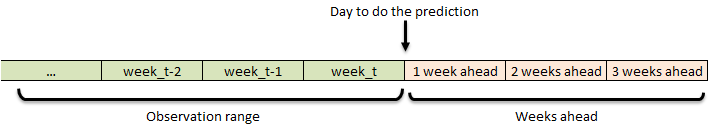
\includegraphics[scale=.7]{Usado_2017-04-30_Weeks_Patrones}
 \caption{Week patterns explanation process} 
 \label{figura8} 
\end{figure}
%

\item Techniques: Se utilizaron las siguientes técnicas, revisando el espacio
paramétrico especificado a continuación:
\begin{itemize}
\item SVR with linear kernel: $C$ $[0.001, 1, 10, 100, 1000]$, $epsilon$ $[0.0, 0.4, 0.9]$.
\item SVR with gaussian kernel: $C$ $[0.001, 1, 10, 100, 1000]$, $epsilon$ $[0.0, 0.4, 0.9]$,
$gamma$ $[0.0, 0.4, 0.9]$.
\item SVR with sigmoid kernel: $C$ $[0.001, 1, 10, 100, 1000]$, $epsilon$ $[0.0, 0.4, 0.9]$,
$gamma$ $[0.0, 0.4, 0.9]$, $coef0$ $[0.0, 0.5, 5, 10]$.
\item Echo state networks: $LeakingRate$ $[0.02 .. 0.9]$, $neurons$ $[1\% .. 90\%]$ de la 
cardinalidad del training set, $InitLen$ $[ 0.1 .. 0.8 ]$.
\item Ordinary least squares linear regression: No parameters.
\item Elastic-net regression: $alpha$ $[0 .. 0.9]$, $l1\_ratio$ $[0 .. 1.0]$.
\end{itemize}

\item Variables included in the model:
\begin{itemize}
\item All variables.
\item From the set $\{ \overline{T}_{a} , \overline{H}, P ,
  \overline{W} \}$ use the subsets with one, two, three or four
  elements. These variables have the largest impact on the disease
  development \citep{MarinVargas1995}.
\end{itemize}
\end{itemize}
